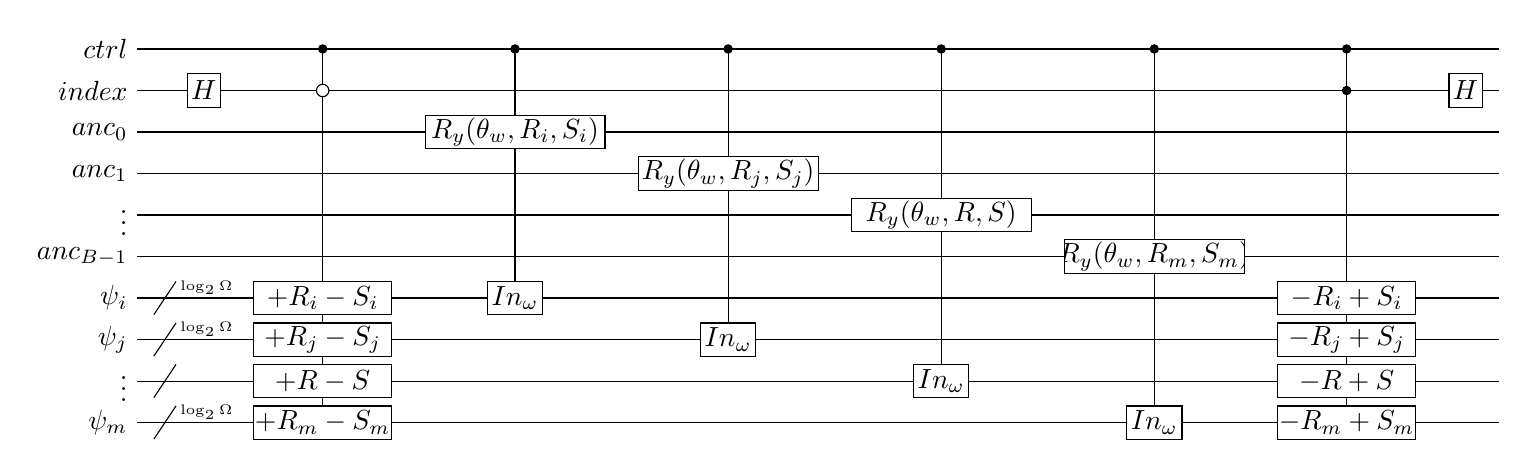
\begin{tikzpicture}[scale=1.000000,x=1pt,y=1pt]
\filldraw[color=white] (0.000000, -7.500000) rectangle (492.000000, 142.500000);
% Drawing wires
% Line 1: ctrl W ctrl
\draw[color=black] (0.000000,135.000000) -- (492.000000,135.000000);
\draw[color=black] (0.000000,135.000000) node[left] {$ctrl$};
% Line 2: index W index
\draw[color=black] (0.000000,120.000000) -- (492.000000,120.000000);
\draw[color=black] (0.000000,120.000000) node[left] {$index$};
% Line 3: anc_0 W anc_0
\draw[color=black] (0.000000,105.000000) -- (492.000000,105.000000);
\draw[color=black] (0.000000,105.000000) node[left] {$anc_0$};
% Line 4: anc_1 W anc_1
\draw[color=black] (0.000000,90.000000) -- (492.000000,90.000000);
\draw[color=black] (0.000000,90.000000) node[left] {$anc_1$};
% Line 5: anc_series W \vdots
\draw[color=black] (0.000000,75.000000) -- (492.000000,75.000000);
\draw[color=black] (0.000000,75.000000) node[left] {$\vdots$};
% Line 6: anc_B W anc_{B-1}
\draw[color=black] (0.000000,60.000000) -- (492.000000,60.000000);
\draw[color=black] (0.000000,60.000000) node[left] {$anc_{B-1}$};
% Line 8: i W \psi_i
\draw[color=black] (0.000000,45.000000) -- (492.000000,45.000000);
\draw[color=black] (0.000000,45.000000) node[left] {$\psi_i$};
% Line 9: j W \psi_j
\draw[color=black] (0.000000,30.000000) -- (492.000000,30.000000);
\draw[color=black] (0.000000,30.000000) node[left] {$\psi_j$};
% Line 10: sys_series W \vdots
\draw[color=black] (0.000000,15.000000) -- (492.000000,15.000000);
\draw[color=black] (0.000000,15.000000) node[left] {$\vdots$};
% Line 11: m W \psi_m
\draw[color=black] (0.000000,0.000000) -- (492.000000,0.000000);
\draw[color=black] (0.000000,0.000000) node[left] {$\psi_m$};
% Done with wires; drawing gates
% Line 13: i / ^{\log_2{\Omega}}
\draw (6.000000, 39.000000) -- (14.000000, 51.000000);
\draw (12.000000, 48.000000) node[right] {$\scriptstyle{^{\log_2{\Omega}}}$};
% Line 14: j / ^{\log_2{\Omega}}
\draw (6.000000, 24.000000) -- (14.000000, 36.000000);
\draw (12.000000, 33.000000) node[right] {$\scriptstyle{^{\log_2{\Omega}}}$};
% Line 15: sys_series /
\draw (6.000000, 9.000000) -- (14.000000, 21.000000);
% Line 16: m / ^{\log_2{\Omega}}
\draw (6.000000, -6.000000) -- (14.000000, 6.000000);
\draw (12.000000, 3.000000) node[right] {$\scriptstyle{^{\log_2{\Omega}}}$};
% Line 18: ctrl index anc_0 anc_1 anc_series anc_B i j sys_series m LABEL width=-20
% Line 20: index G $H$
\begin{scope}
\draw[fill=white] (24.000000, 120.000000) +(-45.000000:8.485281pt and 8.485281pt) -- +(45.000000:8.485281pt and 8.485281pt) -- +(135.000000:8.485281pt and 8.485281pt) -- +(225.000000:8.485281pt and 8.485281pt) -- cycle;
\clip (24.000000, 120.000000) +(-45.000000:8.485281pt and 8.485281pt) -- +(45.000000:8.485281pt and 8.485281pt) -- +(135.000000:8.485281pt and 8.485281pt) -- +(225.000000:8.485281pt and 8.485281pt) -- cycle;
\draw (24.000000, 120.000000) node {$H$};
\end{scope}
% Line 22: i G width=50 $+R_i-S_i$ j G width=50 $+R_j-S_j$ sys_series G width=50 $+R-S$ m G width=50 $+R_m-S_m$ ctrl -index
\draw (67.000000,135.000000) -- (67.000000,0.000000);
\begin{scope}
\draw[fill=white] (67.000000, 45.000000) +(-45.000000:35.355339pt and 8.485281pt) -- +(45.000000:35.355339pt and 8.485281pt) -- +(135.000000:35.355339pt and 8.485281pt) -- +(225.000000:35.355339pt and 8.485281pt) -- cycle;
\clip (67.000000, 45.000000) +(-45.000000:35.355339pt and 8.485281pt) -- +(45.000000:35.355339pt and 8.485281pt) -- +(135.000000:35.355339pt and 8.485281pt) -- +(225.000000:35.355339pt and 8.485281pt) -- cycle;
\draw (67.000000, 45.000000) node {$+R_i-S_i$};
\end{scope}
\begin{scope}
\draw[fill=white] (67.000000, 30.000000) +(-45.000000:35.355339pt and 8.485281pt) -- +(45.000000:35.355339pt and 8.485281pt) -- +(135.000000:35.355339pt and 8.485281pt) -- +(225.000000:35.355339pt and 8.485281pt) -- cycle;
\clip (67.000000, 30.000000) +(-45.000000:35.355339pt and 8.485281pt) -- +(45.000000:35.355339pt and 8.485281pt) -- +(135.000000:35.355339pt and 8.485281pt) -- +(225.000000:35.355339pt and 8.485281pt) -- cycle;
\draw (67.000000, 30.000000) node {$+R_j-S_j$};
\end{scope}
\begin{scope}
\draw[fill=white] (67.000000, 15.000000) +(-45.000000:35.355339pt and 8.485281pt) -- +(45.000000:35.355339pt and 8.485281pt) -- +(135.000000:35.355339pt and 8.485281pt) -- +(225.000000:35.355339pt and 8.485281pt) -- cycle;
\clip (67.000000, 15.000000) +(-45.000000:35.355339pt and 8.485281pt) -- +(45.000000:35.355339pt and 8.485281pt) -- +(135.000000:35.355339pt and 8.485281pt) -- +(225.000000:35.355339pt and 8.485281pt) -- cycle;
\draw (67.000000, 15.000000) node {$+R-S$};
\end{scope}
\begin{scope}
\draw[fill=white] (67.000000, -0.000000) +(-45.000000:35.355339pt and 8.485281pt) -- +(45.000000:35.355339pt and 8.485281pt) -- +(135.000000:35.355339pt and 8.485281pt) -- +(225.000000:35.355339pt and 8.485281pt) -- cycle;
\clip (67.000000, -0.000000) +(-45.000000:35.355339pt and 8.485281pt) -- +(45.000000:35.355339pt and 8.485281pt) -- +(135.000000:35.355339pt and 8.485281pt) -- +(225.000000:35.355339pt and 8.485281pt) -- cycle;
\draw (67.000000, -0.000000) node {$+R_m-S_m$};
\end{scope}
\filldraw (67.000000, 135.000000) circle(1.500000pt);
\draw[fill=white] (67.000000, 120.000000) circle(2.250000pt);
% Line 24: anc_0 G:width=65 $R_y(\theta_w, R_i, S_i)$ i G:width=20 $In_\omega$ ctrl
\draw (136.500000,135.000000) -- (136.500000,45.000000);
\begin{scope}
\draw[fill=white] (136.500000, 105.000000) +(-45.000000:45.961941pt and 8.485281pt) -- +(45.000000:45.961941pt and 8.485281pt) -- +(135.000000:45.961941pt and 8.485281pt) -- +(225.000000:45.961941pt and 8.485281pt) -- cycle;
\clip (136.500000, 105.000000) +(-45.000000:45.961941pt and 8.485281pt) -- +(45.000000:45.961941pt and 8.485281pt) -- +(135.000000:45.961941pt and 8.485281pt) -- +(225.000000:45.961941pt and 8.485281pt) -- cycle;
\draw (136.500000, 105.000000) node {$R_y(\theta_w, R_i, S_i)$};
\end{scope}
\begin{scope}
\draw[fill=white] (136.500000, 45.000000) +(-45.000000:14.142136pt and 8.485281pt) -- +(45.000000:14.142136pt and 8.485281pt) -- +(135.000000:14.142136pt and 8.485281pt) -- +(225.000000:14.142136pt and 8.485281pt) -- cycle;
\clip (136.500000, 45.000000) +(-45.000000:14.142136pt and 8.485281pt) -- +(45.000000:14.142136pt and 8.485281pt) -- +(135.000000:14.142136pt and 8.485281pt) -- +(225.000000:14.142136pt and 8.485281pt) -- cycle;
\draw (136.500000, 45.000000) node {$In_\omega$};
\end{scope}
\filldraw (136.500000, 135.000000) circle(1.500000pt);
% Line 25: anc_1 G:width=65 $R_y(\theta_w, R_j, S_j)$ j G:width=20 $In_\omega$ ctrl
\draw (213.500000,135.000000) -- (213.500000,30.000000);
\begin{scope}
\draw[fill=white] (213.500000, 90.000000) +(-45.000000:45.961941pt and 8.485281pt) -- +(45.000000:45.961941pt and 8.485281pt) -- +(135.000000:45.961941pt and 8.485281pt) -- +(225.000000:45.961941pt and 8.485281pt) -- cycle;
\clip (213.500000, 90.000000) +(-45.000000:45.961941pt and 8.485281pt) -- +(45.000000:45.961941pt and 8.485281pt) -- +(135.000000:45.961941pt and 8.485281pt) -- +(225.000000:45.961941pt and 8.485281pt) -- cycle;
\draw (213.500000, 90.000000) node {$R_y(\theta_w, R_j, S_j)$};
\end{scope}
\begin{scope}
\draw[fill=white] (213.500000, 30.000000) +(-45.000000:14.142136pt and 8.485281pt) -- +(45.000000:14.142136pt and 8.485281pt) -- +(135.000000:14.142136pt and 8.485281pt) -- +(225.000000:14.142136pt and 8.485281pt) -- cycle;
\clip (213.500000, 30.000000) +(-45.000000:14.142136pt and 8.485281pt) -- +(45.000000:14.142136pt and 8.485281pt) -- +(135.000000:14.142136pt and 8.485281pt) -- +(225.000000:14.142136pt and 8.485281pt) -- cycle;
\draw (213.500000, 30.000000) node {$In_\omega$};
\end{scope}
\filldraw (213.500000, 135.000000) circle(1.500000pt);
% Line 26: anc_series G:width=65 $R_y(\theta_w, R, S)$ sys_series G:width=20 $In_\omega$ ctrl
\draw (290.500000,135.000000) -- (290.500000,15.000000);
\begin{scope}
\draw[fill=white] (290.500000, 75.000000) +(-45.000000:45.961941pt and 8.485281pt) -- +(45.000000:45.961941pt and 8.485281pt) -- +(135.000000:45.961941pt and 8.485281pt) -- +(225.000000:45.961941pt and 8.485281pt) -- cycle;
\clip (290.500000, 75.000000) +(-45.000000:45.961941pt and 8.485281pt) -- +(45.000000:45.961941pt and 8.485281pt) -- +(135.000000:45.961941pt and 8.485281pt) -- +(225.000000:45.961941pt and 8.485281pt) -- cycle;
\draw (290.500000, 75.000000) node {$R_y(\theta_w, R, S)$};
\end{scope}
\begin{scope}
\draw[fill=white] (290.500000, 15.000000) +(-45.000000:14.142136pt and 8.485281pt) -- +(45.000000:14.142136pt and 8.485281pt) -- +(135.000000:14.142136pt and 8.485281pt) -- +(225.000000:14.142136pt and 8.485281pt) -- cycle;
\clip (290.500000, 15.000000) +(-45.000000:14.142136pt and 8.485281pt) -- +(45.000000:14.142136pt and 8.485281pt) -- +(135.000000:14.142136pt and 8.485281pt) -- +(225.000000:14.142136pt and 8.485281pt) -- cycle;
\draw (290.500000, 15.000000) node {$In_\omega$};
\end{scope}
\filldraw (290.500000, 135.000000) circle(1.500000pt);
% Line 27: anc_B G:width=65 $R_y(\theta_w, R_m, S_m)$ m G:width=20 $In_\omega$ ctrl
\draw (367.500000,135.000000) -- (367.500000,0.000000);
\begin{scope}
\draw[fill=white] (367.500000, 60.000000) +(-45.000000:45.961941pt and 8.485281pt) -- +(45.000000:45.961941pt and 8.485281pt) -- +(135.000000:45.961941pt and 8.485281pt) -- +(225.000000:45.961941pt and 8.485281pt) -- cycle;
\clip (367.500000, 60.000000) +(-45.000000:45.961941pt and 8.485281pt) -- +(45.000000:45.961941pt and 8.485281pt) -- +(135.000000:45.961941pt and 8.485281pt) -- +(225.000000:45.961941pt and 8.485281pt) -- cycle;
\draw (367.500000, 60.000000) node {$R_y(\theta_w, R_m, S_m)$};
\end{scope}
\begin{scope}
\draw[fill=white] (367.500000, -0.000000) +(-45.000000:14.142136pt and 8.485281pt) -- +(45.000000:14.142136pt and 8.485281pt) -- +(135.000000:14.142136pt and 8.485281pt) -- +(225.000000:14.142136pt and 8.485281pt) -- cycle;
\clip (367.500000, -0.000000) +(-45.000000:14.142136pt and 8.485281pt) -- +(45.000000:14.142136pt and 8.485281pt) -- +(135.000000:14.142136pt and 8.485281pt) -- +(225.000000:14.142136pt and 8.485281pt) -- cycle;
\draw (367.500000, -0.000000) node {$In_\omega$};
\end{scope}
\filldraw (367.500000, 135.000000) circle(1.500000pt);
% Line 29: i G width=50 $-R_i+S_i$ j G width=50 $-R_j+S_j$ sys_series G width=50 $-R+S$ m G width=50 $-R_m+S_m$ ctrl index
\draw (437.000000,135.000000) -- (437.000000,0.000000);
\begin{scope}
\draw[fill=white] (437.000000, 45.000000) +(-45.000000:35.355339pt and 8.485281pt) -- +(45.000000:35.355339pt and 8.485281pt) -- +(135.000000:35.355339pt and 8.485281pt) -- +(225.000000:35.355339pt and 8.485281pt) -- cycle;
\clip (437.000000, 45.000000) +(-45.000000:35.355339pt and 8.485281pt) -- +(45.000000:35.355339pt and 8.485281pt) -- +(135.000000:35.355339pt and 8.485281pt) -- +(225.000000:35.355339pt and 8.485281pt) -- cycle;
\draw (437.000000, 45.000000) node {$-R_i+S_i$};
\end{scope}
\begin{scope}
\draw[fill=white] (437.000000, 30.000000) +(-45.000000:35.355339pt and 8.485281pt) -- +(45.000000:35.355339pt and 8.485281pt) -- +(135.000000:35.355339pt and 8.485281pt) -- +(225.000000:35.355339pt and 8.485281pt) -- cycle;
\clip (437.000000, 30.000000) +(-45.000000:35.355339pt and 8.485281pt) -- +(45.000000:35.355339pt and 8.485281pt) -- +(135.000000:35.355339pt and 8.485281pt) -- +(225.000000:35.355339pt and 8.485281pt) -- cycle;
\draw (437.000000, 30.000000) node {$-R_j+S_j$};
\end{scope}
\begin{scope}
\draw[fill=white] (437.000000, 15.000000) +(-45.000000:35.355339pt and 8.485281pt) -- +(45.000000:35.355339pt and 8.485281pt) -- +(135.000000:35.355339pt and 8.485281pt) -- +(225.000000:35.355339pt and 8.485281pt) -- cycle;
\clip (437.000000, 15.000000) +(-45.000000:35.355339pt and 8.485281pt) -- +(45.000000:35.355339pt and 8.485281pt) -- +(135.000000:35.355339pt and 8.485281pt) -- +(225.000000:35.355339pt and 8.485281pt) -- cycle;
\draw (437.000000, 15.000000) node {$-R+S$};
\end{scope}
\begin{scope}
\draw[fill=white] (437.000000, -0.000000) +(-45.000000:35.355339pt and 8.485281pt) -- +(45.000000:35.355339pt and 8.485281pt) -- +(135.000000:35.355339pt and 8.485281pt) -- +(225.000000:35.355339pt and 8.485281pt) -- cycle;
\clip (437.000000, -0.000000) +(-45.000000:35.355339pt and 8.485281pt) -- +(45.000000:35.355339pt and 8.485281pt) -- +(135.000000:35.355339pt and 8.485281pt) -- +(225.000000:35.355339pt and 8.485281pt) -- cycle;
\draw (437.000000, -0.000000) node {$-R_m+S_m$};
\end{scope}
\filldraw (437.000000, 135.000000) circle(1.500000pt);
\filldraw (437.000000, 120.000000) circle(1.500000pt);
% Line 31: index G $H$
\begin{scope}
\draw[fill=white] (480.000000, 120.000000) +(-45.000000:8.485281pt and 8.485281pt) -- +(45.000000:8.485281pt and 8.485281pt) -- +(135.000000:8.485281pt and 8.485281pt) -- +(225.000000:8.485281pt and 8.485281pt) -- cycle;
\clip (480.000000, 120.000000) +(-45.000000:8.485281pt and 8.485281pt) -- +(45.000000:8.485281pt and 8.485281pt) -- +(135.000000:8.485281pt and 8.485281pt) -- +(225.000000:8.485281pt and 8.485281pt) -- cycle;
\draw (480.000000, 120.000000) node {$H$};
\end{scope}
% Done with gates; drawing ending labels
% Done with ending labels; drawing cut lines and comments
% Done with comments
\end{tikzpicture}
